\documentclass[]{article}
\usepackage{lmodern}
\usepackage{amssymb,amsmath}
\usepackage{ifxetex,ifluatex}
\usepackage{fixltx2e} % provides \textsubscript
\ifnum 0\ifxetex 1\fi\ifluatex 1\fi=0 % if pdftex
  \usepackage[T1]{fontenc}
  \usepackage[utf8]{inputenc}
\else % if luatex or xelatex
  \ifxetex
    \usepackage{mathspec}
  \else
    \usepackage{fontspec}
  \fi
  \defaultfontfeatures{Ligatures=TeX,Scale=MatchLowercase}
\fi
% use upquote if available, for straight quotes in verbatim environments
\IfFileExists{upquote.sty}{\usepackage{upquote}}{}
% use microtype if available
\IfFileExists{microtype.sty}{%
\usepackage{microtype}
\UseMicrotypeSet[protrusion]{basicmath} % disable protrusion for tt fonts
}{}
\usepackage[margin=1in]{geometry}
\usepackage{hyperref}
\hypersetup{unicode=true,
            pdftitle={Prediction of NBA Player's Salary Based on Stepwise Regression Model},
            pdfauthor={Hongye Xu},
            pdfborder={0 0 0},
            breaklinks=true}
\urlstyle{same}  % don't use monospace font for urls
\usepackage{longtable,booktabs}
\usepackage{graphicx,grffile}
\makeatletter
\def\maxwidth{\ifdim\Gin@nat@width>\linewidth\linewidth\else\Gin@nat@width\fi}
\def\maxheight{\ifdim\Gin@nat@height>\textheight\textheight\else\Gin@nat@height\fi}
\makeatother
% Scale images if necessary, so that they will not overflow the page
% margins by default, and it is still possible to overwrite the defaults
% using explicit options in \includegraphics[width, height, ...]{}
\setkeys{Gin}{width=\maxwidth,height=\maxheight,keepaspectratio}
\IfFileExists{parskip.sty}{%
\usepackage{parskip}
}{% else
\setlength{\parindent}{0pt}
\setlength{\parskip}{6pt plus 2pt minus 1pt}
}
\setlength{\emergencystretch}{3em}  % prevent overfull lines
\providecommand{\tightlist}{%
  \setlength{\itemsep}{0pt}\setlength{\parskip}{0pt}}
\setcounter{secnumdepth}{0}
% Redefines (sub)paragraphs to behave more like sections
\ifx\paragraph\undefined\else
\let\oldparagraph\paragraph
\renewcommand{\paragraph}[1]{\oldparagraph{#1}\mbox{}}
\fi
\ifx\subparagraph\undefined\else
\let\oldsubparagraph\subparagraph
\renewcommand{\subparagraph}[1]{\oldsubparagraph{#1}\mbox{}}
\fi

%%% Use protect on footnotes to avoid problems with footnotes in titles
\let\rmarkdownfootnote\footnote%
\def\footnote{\protect\rmarkdownfootnote}

%%% Change title format to be more compact
\usepackage{titling}

% Create subtitle command for use in maketitle
\newcommand{\subtitle}[1]{
  \posttitle{
    \begin{center}\large#1\end{center}
    }
}

\setlength{\droptitle}{-2em}

  \title{Prediction of NBA Player's Salary Based on Stepwise Regression Model}
    \pretitle{\vspace{\droptitle}\centering\huge}
  \posttitle{\par}
    \author{Hongye Xu}
    \preauthor{\centering\large\emph}
  \postauthor{\par}
    \date{}
    \predate{}\postdate{}
  

\begin{document}
\maketitle

\begin{center}\rule{0.5\linewidth}{\linethickness}\end{center}

\section{1 Introduction}\label{introduction}

\subsection{1.1 Background}\label{background}

I have always felt that the NBA has the best data storage in the sport
filed. In the beginning, I wanted to analyze the performance of the
players by scrapping the data from the official NBA.stat website.
However, since the NBA.stat table is in javascript format, and the
official has canceled all the existing official APIs, no possible
R-based crawler method has been found after the effort. Therefore, I
chose an alternative, which is the basketball-reference website. This
report is based on two data sources on the basketball-reference. My goal
is to predict the player's salary for next season based on player
performance this season.

\subsection{1.2 Glossary}\label{glossary}

\begin{longtable}[]{@{}ll@{}}
\toprule
Abbreviation & Explanation\tabularnewline
\midrule
\endhead
Pos & Position\tabularnewline
Age & Age of Player at the start of February 1st of that
season\tabularnewline
Tm & Team\tabularnewline
G & Games\tabularnewline
GS & Games Started\tabularnewline
MP & Minutes Played Per Game\tabularnewline
FG & Field Goals Per Game\tabularnewline
FGA & Field Goal Attempts Per Game\tabularnewline
FG\% & Field Goal Percentage\tabularnewline
3P & 3-Point Field Goals Per Game\tabularnewline
3PA & 3-Point Field Goal Attempts Per Game\tabularnewline
3P\% & FG\% on 3-Pt FGAs.\tabularnewline
2P & 2-Point Field Goals Per Game\tabularnewline
2PA & 2-Point Field Goal Attempts Per Game\tabularnewline
eFG\% & Effective Field Goal Percentage\tabularnewline
FT & Free Throws Per Game\tabularnewline
FTA & Free Throw Attempts Per Game\tabularnewline
FT\% & Free Throw Percentage\tabularnewline
ORB & Offensive Rebounds Per Game\tabularnewline
DRB & Defensive Rebounds Per Game\tabularnewline
TRB & Total Rebounds Per Game\tabularnewline
AST & Assists Per Game\tabularnewline
STL & Steals Per Game\tabularnewline
BLK & Blocks Per Game\tabularnewline
TOV & Turnovers Per Game\tabularnewline
PF & Personal Fouls Per Game\tabularnewline
PTS & Points Per Game\tabularnewline
\bottomrule
\end{longtable}

\section{2 Preparation}\label{preparation}

\subsection{2.1 Data Scraping and
Cleaning}\label{data-scraping-and-cleaning}

\subsubsection{2.1.1 Players' Regular Season
Data}\label{players-regular-season-data}

My first data source came from
\url{https://www.basketball-reference.com/leagues/NBA_2019_per_game.html}.
Because all the data in the website is displayed in the form of HTML
table, I can read the data in this table by reading the
XPath('//*{[}@id="per\_game\_stats"{]}') of the table with Chrome
browser. At the same time, because many NBA players transfer during the
season, this data source records their data in many teams, and we just
need to keep the data that represents their season average.In addition,
I deleted those rows which do not contain 3 points field goals, 2 points
field goals and free throw field goals.

\begin{verbatim}
##         Player Pos Age  Tm  G GS   MP  FG  FGA   FG%  3P 3PA   3P%  2P
## 1 Alex Abrines  SG  25 OKC 31  2 19.0 1.8  5.1 0.357 1.3 4.1 0.323 0.5
## 2   Quincy Acy  PF  28 PHO 10  0 12.3 0.4  1.8 0.222 0.2 1.5 0.133 0.2
## 3 Jaylen Adams  PG  22 ATL 34  1 12.6 1.1  3.2 0.345 0.7 2.2 0.338 0.4
## 4 Steven Adams   C  25 OKC 80 80 33.4 6.0 10.1 0.595 0.0 0.0 0.000 6.0
## 5  Bam Adebayo   C  21 MIA 82 28 23.3 3.4  5.9 0.576 0.0 0.2 0.200 3.4
## 6    Deng Adel  SF  21 CLE 19  3 10.2 0.6  1.9 0.306 0.3 1.2 0.261 0.3
##    2PA   2P%  eFG%  FT FTA   FT% ORB DRB TRB AST STL BLK TOV  PF  PTS
## 1  1.0 0.500 0.487 0.4 0.4 0.923 0.2 1.4 1.5 0.6 0.5 0.2 0.5 1.7  5.3
## 2  0.3 0.667 0.278 0.7 1.0 0.700 0.3 2.2 2.5 0.8 0.1 0.4 0.4 2.4  1.7
## 3  1.1 0.361 0.459 0.2 0.3 0.778 0.3 1.4 1.8 1.9 0.4 0.1 0.8 1.3  3.2
## 4 10.1 0.596 0.595 1.8 3.7 0.500 4.9 4.6 9.5 1.6 1.5 1.0 1.7 2.6 13.9
## 5  5.7 0.588 0.579 2.0 2.8 0.735 2.0 5.3 7.3 2.2 0.9 0.8 1.5 2.5  8.9
## 6  0.7 0.385 0.389 0.2 0.2 1.000 0.2 0.8 1.0 0.3 0.1 0.2 0.3 0.7  1.7
\end{verbatim}

\subsubsection{2.1.2 Scale}\label{scale}

Considering that regression analysis is mainly used in this report. In
order to eliminate the inaccuracy of parameters caused by too large or
too small data itself. I create a standardized version of the data.

\begin{verbatim}
##                     Age         MP         2P%        3P%         FT%
## Alex Abrines -0.2348656 -0.1678429 -0.05111731  0.1079674  1.30497350
## Quincy Acy    0.4772268 -0.9471834  2.01348589 -1.5619660 -0.28148044
## Jaylen Adams -0.9469579 -0.9122876 -1.76955950  0.2398043  0.27342273
## Steven Adams -0.2348656  1.5071577  1.13572046 -2.7309194 -1.70430908
## Bam Adebayo  -1.1843221  0.3323309  1.03681731 -0.9730947 -0.03248542
## Deng Adel    -1.1843221 -1.1914543 -1.47285006 -0.4369582  1.85276253
##                     TRB         AST        STL         BLK        TOV
## Alex Abrines -0.9119870 -0.81732136 -0.3701968 -0.49747590 -0.7975707
## Quincy Acy   -0.4970106 -0.70641502 -1.3498261  0.02415998 -0.9238106
## Jaylen Adams -0.7874941 -0.09643014 -0.6151041 -0.75829384 -0.4188509
## Steven Adams  2.4078238 -0.26278966  2.0788766  1.58906762  0.7173087
## Bam Adebayo   1.4948758  0.06992937  0.6094326  1.06743174  0.4648288
## Deng Adel    -1.1194751 -0.98368087 -1.3498261 -0.49747590 -1.0500506
##                      PF         PTS
## Alex Abrines -0.1395071 -0.64209057
## Quincy Acy    0.7994827 -1.23613639
## Jaylen Adams -0.6760726 -0.98861730
## Steven Adams  1.0677655  0.77701887
## Bam Adebayo   0.9336241 -0.04804476
## Deng Adel    -1.4809210 -1.23613639
\end{verbatim}

\subsubsection{2.1.3 Players' Salaries}\label{players-salaries}

The second data came from
\url{https://www.basketball-reference.com/contracts/players.html}, and I
imported it in the same way as I scrapped the first data. This data
includes salary data for the next six seasons. But all we need is this
season's data, so I filtered it and converted character data into
numeric data. The result is as follow.

\begin{verbatim}
## [1] Player             Tm                 2018-19           
## [4] duplicated(Player)
## <0 rows> (or 0-length row.names)
\end{verbatim}

\begin{verbatim}
##              Player  Tm  2018-19
## 1     Stephen Curry GSW 37457154
## 2        Chris Paul HOU 35654150
## 3 Russell Westbrook OKC 35654150
## 4      LeBron James LAL 35654150
## 5     Blake Griffin DET 32088932
## 6    Gordon Hayward BOS 31214295
\end{verbatim}

Finally, there is no duplicate player data.

\subsubsection{2.1.4 Merging Data}\label{merging-data}

Merge standardized and non-standardized data with player salary data to
get the final data we need.

\subsubsection{2.1.5 Save No\_scale Data Into
CSV}\label{save-no_scale-data-into-csv}

I saved the merged non-standardized data to the working directory with
the file name'18-19 players\_stat.csv'.

\section{3 Correlation Check}\label{correlation-check}

\subsection{3.1 Frist Check}\label{frist-check}

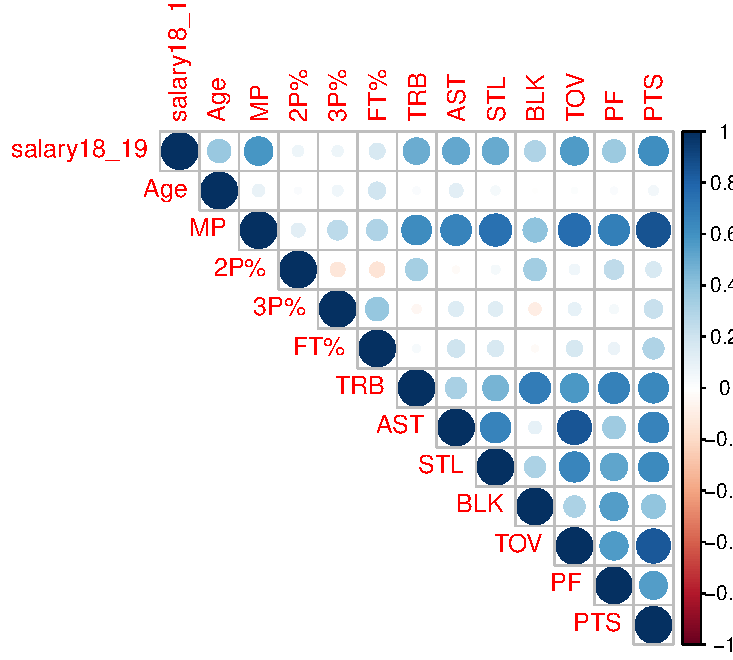
\includegraphics{Final_Report_files/figure-latex/unnamed-chunk-11-1.pdf}

The features that have strong correlation with salary
are:PTS,TOV,STL,AST,TRB and MP. Besides, MP is strongly correlated with
multiple features and may have multiple collinearities(This is in line
with our common sense. The more time we play, the better the data will
be). What I didn't expect was that the correlation between field goal
and salary was not high, that is to say, the output of players
influenced the salary of players more than efficiency.

\subsection{3.2 Second Check}\label{second-check}

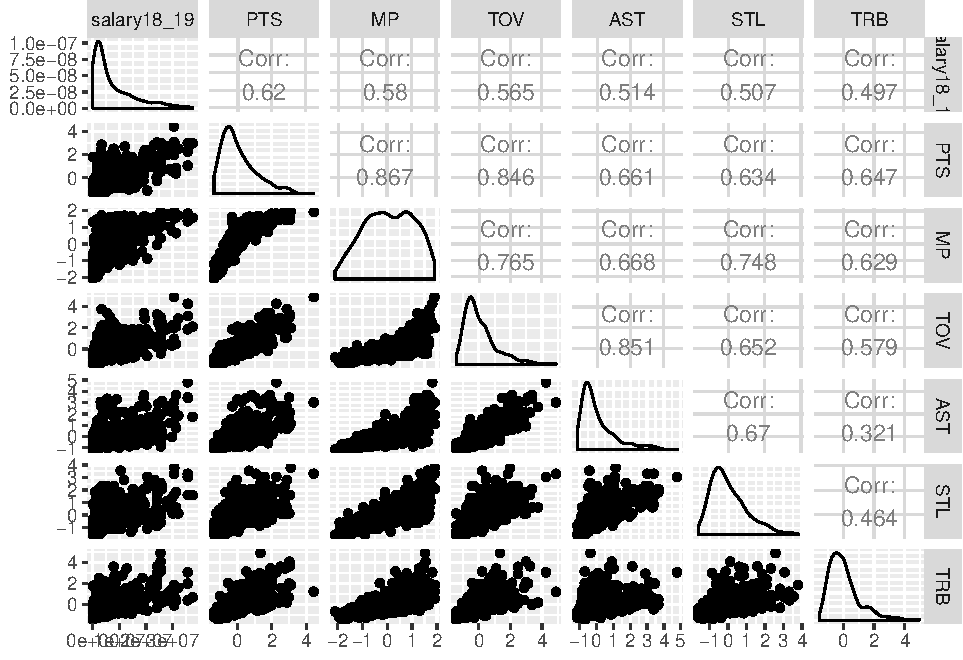
\includegraphics{Final_Report_files/figure-latex/unnamed-chunk-12-1.pdf}

\begin{verbatim}
## salary18_19         PTS          MP         TOV         AST         STL 
##   1.0000000   0.6198192   0.5803967   0.5645525   0.5142283   0.5066299 
##         TRB 
##   0.4972563
\end{verbatim}

Correlation strength is: PTS \textgreater{} MP \textgreater{} TOV
\textgreater{} AST \textgreater{} STL \textgreater{} TRB There's also
one thing that surprises me: the number of players'turnivers is
positively correlated with their salaries. I mean, generally speaking,
assuming that a player's turnover rate is constant, the total number of
turnovers will increase as his minutes played increases, and important
players will have higher minutes played and higher salaries.

\section{4 Data Visualization}\label{data-visualization}

\subsection{4.1 Interactive Plot}\label{interactive-plot}

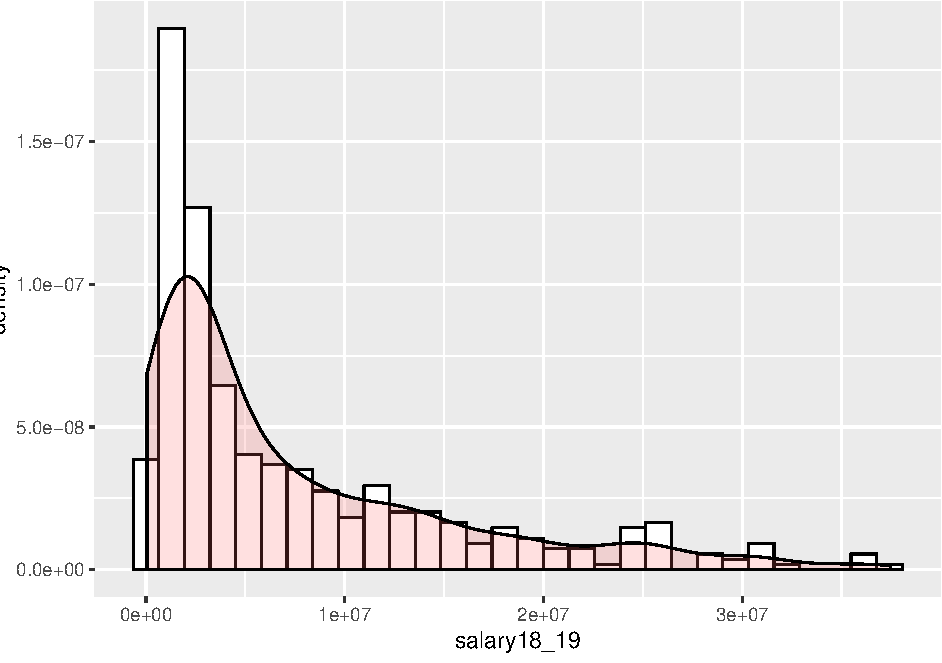
\includegraphics{Final_Report_files/figure-latex/unnamed-chunk-13-1.png}

\subsection{4.2 Scatter Plot With Regression
Line}\label{scatter-plot-with-regression-line}

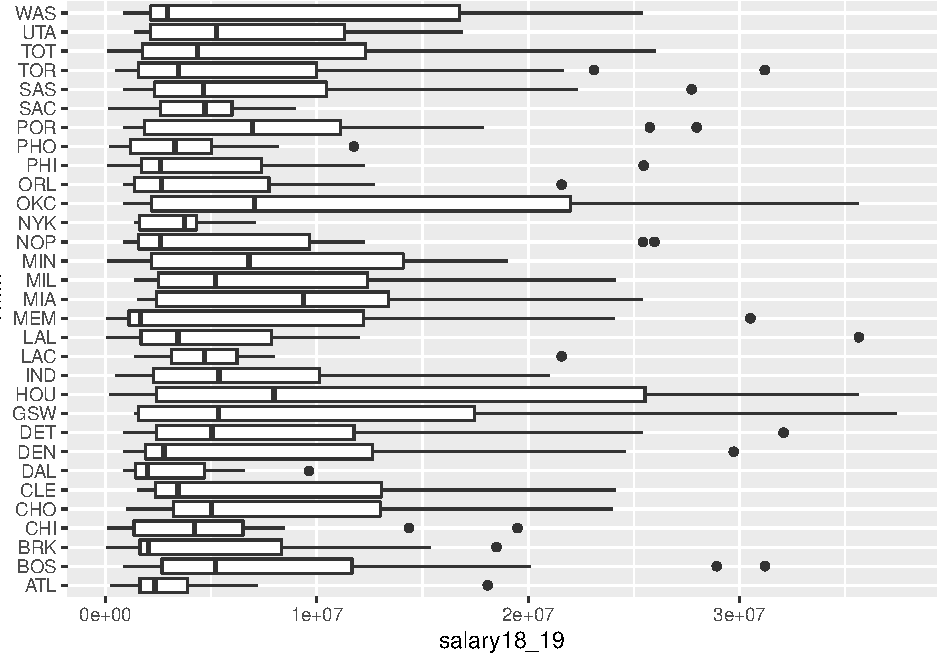
\includegraphics{Final_Report_files/figure-latex/unnamed-chunk-14-1.pdf}

Under the simple linear model, we can understand that the fitted curve
represents the average level of the league, and the player below the
curve performs worse than the expected performance corresponding to the
salary. We can check their name by hovering on the points in the
interactive plot(only in HTML form file). It includes a lot of All-Star
players, such as Chris Paul, Kyle Lowry, Al Horford, Gordon Haywood(The
Celtics are unlucky) and etc. However, it only considers the scoring
feature, and does not fully reflect the players'influence on the field.

\section{5 Multiple Regression}\label{multiple-regression}

\begin{verbatim}
## 
## Call:
## lm(formula = salary18_19 ~ PTS + MP + TOV + AST + STL + TRB, 
##     data = regression)
## 
## Coefficients:
## (Intercept)          PTS           MP          TOV          AST  
##     7114340      3626578      -546186     -2022044      2571555  
##         STL          TRB  
##      833962      1888579
\end{verbatim}

From here, we can see that points per game is the most significant
feature of positive impact, while turnovers per game is the most
significant feature of negative impact. However, simple multiple
regression also has some problems, that is, there are multiple
collinearities.

\subsection{5.1 Player 's Importance And
Incautiousness}\label{player-s-importance-and-incautiousness}

Here we make two definitions that a player is ``important'' if his
minutes played is above average and is ``incautious'' if his turnover
per game is above average.

\subsection{5.2 Prallel Slope Model}\label{prallel-slope-model}

\subsubsection{5.2.1 Incautiousness
Comparision}\label{incautiousness-comparision}

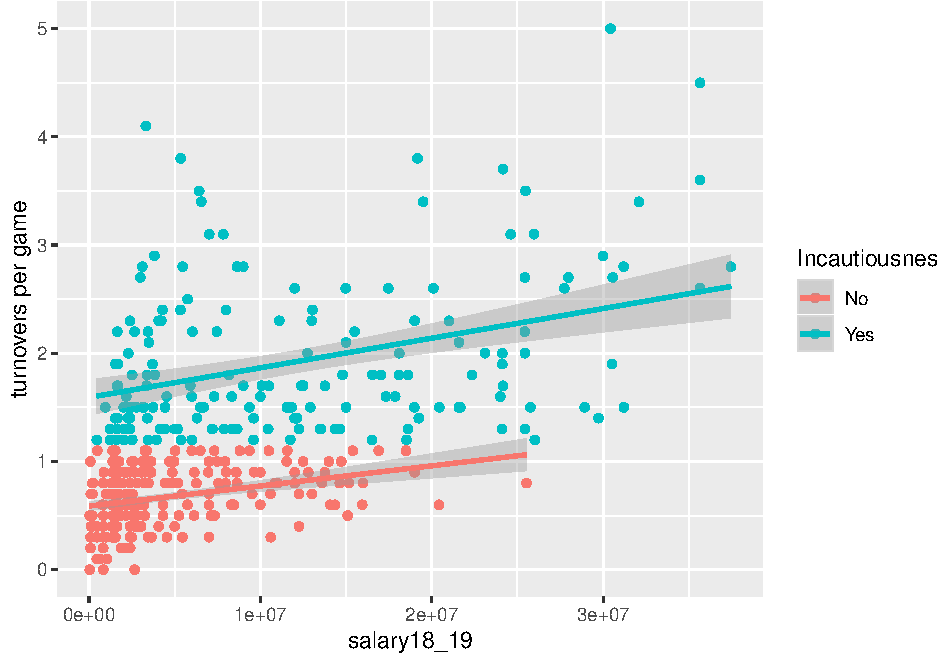
\includegraphics{Final_Report_files/figure-latex/unnamed-chunk-17-1.pdf}

The plot shows that the number of turnovers of the players with higher
salaries will increase correspondingly, but the magnitude is not large.
We can think that it is a natural phenomenon caused by the increase of
playing time. Then I do a regression analysis of Importance and
Incautiousness. The result is as follow

\begin{verbatim}
## 
## Call:
## lm(formula = salary18_19 ~ Importance * Incautiousness, data = regression)
## 
## Coefficients:
##                     (Intercept)                    ImportanceYes  
##                         3275995                          3754147  
##               IncautiousnessYes  ImportanceYes:IncautiousnessYes  
##                         3048670                          3017297
\end{verbatim}

We can assume that the impact of A and B is close to synchronization,
which confirms my previous view that players with higher salaries have
more playing time, which leads to more turnovers, rather than higher
salaries because of higher turnovers.

\subsection{5.3 Stepwise Regression}\label{stepwise-regression}

Considering that the data of NBA players will increase with the increase
of playing time, there must be multiple collinearity among the features.
So stepwise regression is the more accurate method.

\begin{verbatim}
## 
## Call:
## lm(formula = salary18_19 ~ PTS + TOV + AST + STL + TRB, data = regression)
## 
## Residuals:
##       Min        1Q    Median        3Q       Max 
## -15540227  -3515763   -874394   3138553  20906046 
## 
## Coefficients:
##             Estimate Std. Error t value Pr(>|t|)    
## (Intercept)  7101619     295954  23.996  < 2e-16 ***
## PTS          3284754     601916   5.457 8.34e-08 ***
## TOV         -1924931     847259  -2.272 0.023600 *  
## AST          2488319     653919   3.805 0.000163 ***
## STL           679543     437411   1.554 0.121052    
## TRB          1820063     421730   4.316 1.99e-05 ***
## ---
## Signif. codes:  0 '***' 0.001 '**' 0.01 '*' 0.05 '.' 0.1 ' ' 1
## 
## Residual standard error: 6057000 on 415 degrees of freedom
## Multiple R-squared:  0.4391, Adjusted R-squared:  0.4323 
## F-statistic: 64.97 on 5 and 415 DF,  p-value: < 2.2e-16
\end{verbatim}

Here I use k-fold cross-validation to test the error of the models that
have different number of variate.

\begin{verbatim}
##   nvmax    RMSE  Rsquared     MAE   RMSESD RsquaredSD    MAESD
## 1     1 6477031 0.3656265 4841275 740066.8  0.1181143 489025.3
## 2     2 6394271 0.3803728 4800648 640458.4  0.1150337 384294.5
## 3     3 6113242 0.4295432 4634334 621821.6  0.1299230 442098.5
## 4     4 6082951 0.4340008 4636211 662992.5  0.1335307 493985.8
## 5     5 6157695 0.4198971 4707174 644375.1  0.1258431 498597.2
## 6     6 6142967 0.4211164 4689635 668283.2  0.1298739 503369.9
## 7     7 6118851 0.4262623 4685282 678915.2  0.1321880 539508.8
## 8     8 6116129 0.4267740 4683816 673996.1  0.1312854 541582.6
## 9     9 6116129 0.4267740 4683816 673996.1  0.1312854 541582.6
\end{verbatim}

From the result we can see that three-variable model's RMSE is the
smallest and Rsquared is second largest. So the three-variable model is
the best one. Let us find out the order in which variables are added to
the model.

\begin{verbatim}
## Subset selection object
## 8 Variables  (and intercept)
##                   Forced in Forced out
## PTS                   FALSE      FALSE
## MP                    FALSE      FALSE
## TOV                   FALSE      FALSE
## AST                   FALSE      FALSE
## STL                   FALSE      FALSE
## TRB                   FALSE      FALSE
## ImportanceYes         FALSE      FALSE
## IncautiousnessYes     FALSE      FALSE
## 1 subsets of each size up to 4
## Selection Algorithm: backward
##          PTS MP  TOV AST STL TRB ImportanceYes IncautiousnessYes
## 1  ( 1 ) "*" " " " " " " " " " " " "           " "              
## 2  ( 1 ) "*" " " " " "*" " " " " " "           " "              
## 3  ( 1 ) "*" " " " " "*" " " "*" " "           " "              
## 4  ( 1 ) "*" " " "*" "*" " " "*" " "           " "
\end{verbatim}

\begin{verbatim}
## (Intercept)         PTS         AST         TRB 
##     7095995     2678780     1764352     1642389
\end{verbatim}

The best model is salary18\_19 \textasciitilde{} PTS + AST + TRB

\section{6 Conclusion}\label{conclusion}

\subsection{6.1 What i want to predict}\label{what-i-want-to-predict}

As Lebron James fan, I am concerned about the new contract for the
Lakers who may stay next season. Let's find them first.

\begin{verbatim}
## # A tibble: 8 x 1
## # Groups:   Player [8]
##   Player                  
##   <chr>                   
## 1 Kentavious Caldwell-Pope
## 2 Rajon Rondo             
## 3 Mike Muscala            
## 4 Lance Stephenson        
## 5 Reggie Bullock          
## 6 JaVale McGee            
## 7 Andre Ingram            
## 8 Scott Machado
\end{verbatim}

\subsection{6.2 Analysis conclusion}\label{analysis-conclusion}

\begin{verbatim}
## [1] "Expected Salary: $6,771,542"
\end{verbatim}

\begin{verbatim}
## [1] "Expected Salary: $7,275,901"
\end{verbatim}

\begin{verbatim}
## [1] "Expected Salary: $5,902,181"
\end{verbatim}

Here I choose three players who are more likely to stay next season to
make predictions.The result shows that salaries for Pope, Bullock and
Stephenson for next season are \$6,771,542, \$7,275,901 and \$5,902,181

\section{7 Github Link}\label{github-link}

\url{https://github.com/szxuhongye/NBA-Player-Salary-Predicton.git}


\end{document}
